\documentclass[11pt, oneside]{article} 
\usepackage{geometry}
\geometry{letterpaper} 
\usepackage{graphicx}
	
\usepackage{amssymb}
\usepackage{amsmath}
\usepackage{parskip}
\usepackage{color}
\usepackage{hyperref}

\graphicspath{{/Users/telliott_admin/Tex/png/}}
% \begin{center} 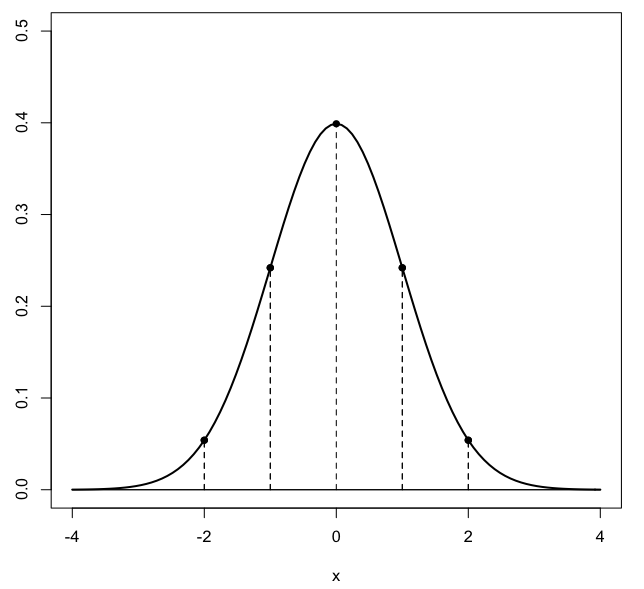
\includegraphics [scale=0.4] {gauss3.png} \end{center}

%break
\title{Optimization problems}
\date{}

\begin{document}
\maketitle
\Large

\subsection*{Projectile range}

Suppose we fire a cannon where the ball has velocity $v$ at an angle $\theta$ with the horizon (straight up would be $\pi/2$ radians).  We wish to determine the angle that will give the maximum range.  We did this problem in a physics section, but it won't hurt to look at it again here.

The problem has a trick, namely that the distance in the horizontal or $x$-direction depends on the time (and therefore distance) in the $y$-direction, since when $y=0$, the cannonball will fall to earth and not move any more.

If you draw a diagram you will see that 
\[ v_y = v \sin \theta \]
where $v_y$ is the initial velocity in the $y$-direction.

The basic equation of motion under gravity is that 
\[ y = v_y t - \frac{1}{2}gt^2 \]
with $g=32$ so
\[ y = v_y t - 16t^2 \]

At the point of interest $y=0$ so
\[ 0 = v_y t - 16t^2 \]
\[ v_y t = 16 t^2 \]

This has two solutions, namely $t=0$ (not what we are interested in) and
\[ v_y = 16 t \]
\[ t = \frac{v_y}{16} \]
\[ = \frac{v \sin \theta}{16} \]

On the other hand, the quantity we are really interested in is the distance in the $x$-direction.  Similarly to $v_y$, 

\[ v_x = v \cos \theta \]
\[ x = v_x t = v \cos \theta \ \frac{v \sin \theta}{16} \]
\[ = \frac{v^2}{16} \ \cos \theta \sin \theta \]

This looks a little strange but all it really says is that the range is a function of the angle $\theta$ (and also of the square of the velocity).  If you do dimensional analysis at this point you might also be confused unless you remember that the factor of $16$ has units of meters per second squared.

We take the first derivative and set it equal to zero:

\[ x' = \frac{v^2}{16} \ (\cos^2 \theta - \sin^2 \theta ) = 0 \]

$v = 0$ gives a solution to this equation, but it's not the solution we want.  We want the solution given by

\[ \cos^2 \theta - \sin^2 \theta = 0 \]

The velocity and the gravitational constant have dropped out, which makes sense.  It makes intuitive sense that the angle for maximum range (given a velocity), should not depend on that velocity.

The above expression is zero when $\cos \theta = \sin \theta$.  If you don't see this you can say:

\[ 1 - \sin^2 \theta - \sin^2 \theta = 0 \]
\[ \sin^2 \theta = \frac{1}{2} \]
\[ \sin \theta = \frac{1}{\sqrt{2}} \]
\[ \theta = \frac{\pi}{4} \]

An elevation of $45$ degrees gives the maximum range.

\subsection*{Closest point to a parabola}

Suppose we consider the simple parabola
\[ y = x^2 \]

Our problem is to find the point(s) $(x,y)$ on the parabola that have the shortest distance to $P=(0,1)$.

One possibility is that $(0,0)$ is the minimum.  But it will turn out that it is not, and so there will be two such points, which are symmetrical about the $y-$axis.  Therefore, we consider only $x \ge 0$.

The distance from any point $(x,y)$ to $P=(0,1)$ is
\[ d = \sqrt{(0-x)^2 + (1-y)^2} \]

It is the case that if we minimize $d^2$, we also minimize $d$, so let's rewrite the equation as

\[ D = (0-x)^2 + (1-y)^2 \]
\[ D = x^2 + 1 - 2y + y^2 \]

Now, the constraint is that $y=x^2$ so plugging in we get

\[ D = y + 1 - 2y + y^2 \]
\[ = 1 - y + y^2 \]

Take the first derivative (with respect to $y$) and set it equal to zero:

\[ D' = -1 + 2y = 0 \]
\[ y = \frac{1}{2} \]
\[ x = \frac{1}{\sqrt{2}} \]

Check the actual distance:

\[ d = \sqrt{(0-x)^2 + (1-y)^2} \]
\[ = \sqrt{(\frac{1}{\sqrt{2}})^2 + (1- \frac{1}{2})^2 } \]
\[ = \sqrt{\frac{1}{2} + \frac{1}{4}} \]
\[ = \frac{\sqrt{3}}{2} \]
\[ = 0.866 \]

\[ (x,y) = (\frac{1}{\sqrt{2}}, \frac{1}{2}) \]

Note that $(1/\sqrt{2},1/2)$ is closer to $(0,1)$ than is $(0,0)$, as we said.

The slope of the line from $(0,1)$ to our point $(1/\sqrt{2},1/2)$ is
\[ \frac{\Delta y}{\Delta x} = \frac{1-1/2}{1/\sqrt{2}} = -\frac{1}{\sqrt{2}} \]

The slope of the tangent to the parabola is $2x$, and at $(1/\sqrt{2},1/2)$ it is

\[ m = 2x = 2 \frac{1}{\sqrt{2}} = \sqrt{2} \]

Since the product of the slopes is $-1$, the line corresponding to the minimum distance is perpendicular to the tangent.

The next two problems are about maximizing angles.  They are variants with a slight twist.

\subsection*{Nelson's column}

Nelson's column is a column with a statue of Nelson on top, naturally.  The hero of Trafalgar is honored at London's Trafalgar square.  Here is Acheson's sketch:

\begin{center} 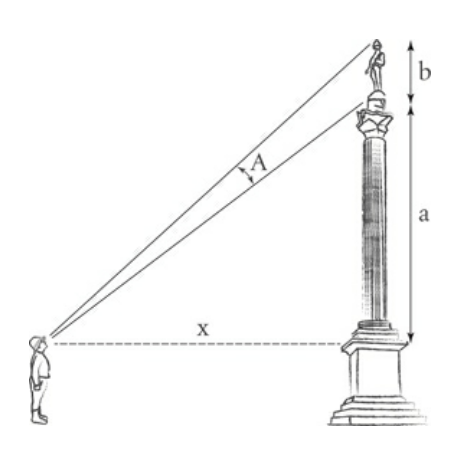
\includegraphics [scale=0.4] {nelson.png} \end{center}

Somehow we need to maximize the angle $A$ as a function of $x$, but we are given values that form the tangent of two angles.

However, we know that for $\theta$ in the half-open interval $[0, \pi/2)$, as $\theta$ increases so does $\tan \theta$.  Therefore, if we maximize $\tan \theta$, $\theta$ will also be a maximum.  This is a standard trick to remember.

Let's use $s$ for the entire angle and $t$ for the lower triangle, then
\[ A = s - t \]
and the lengths we are given can be used to express the tangents of $s$ and $t$.

We derived $\tan s - t$ before, and can do it again:
\[ \tan s - t = \frac{\sin s - t}{\cos s - t} \]
\[ = \frac{\sin s \cos t - \cos s \sin t}{\cos s \cos t + \sin s \sin t} \]
\[ = \frac{\tan s - \tan t}{1 + \tan s \tan t} \]

Plugging in:
\[ \tan A = \frac{\frac{a+b}{x} - \frac{a}{x}}{1 + \frac{a(a+b)}{x^2}} \]
The numerator simplifies to $b/x$, so let's keep the $b$ on top and multiply on the bottom by $x$
\[ \tan A = \frac{b}{x + a(a+b)/x} \]

I got a bit of a mess trying to work with this as it is, so I multiplied by $x$ on top and bottom a second time:
\[ \tan A = \frac{bx}{x^2 + a(a+b)} \]

Use the familiar quotient rule to take the derivative and set it equal to zero:
\[ 0 = \frac{b \ [ \ x^2 + a(a+b) \ ] - bx(2x)}{[ \ x^2 + a(a+b) \ ]^2} \]

This occurs when the numerator is zero so discard the denominator!
\[ 0 = b \ [ \ x^2 + a(a+b) \ ] - bx(2x) \]
Factor out the $b$, put the two terms on opposite sides and obtain
\[ x^2 + a(a + b) = 2x^2 \]
\[ x^2 = a(a+b) \]

This is the solution given in Acheson.  Furthermore, the statue is fairly small compared to the column's height.  If we let $b << a$ then
\[ x^2 \approx a^2 \]
\[ x \approx a \]
The appropriate viewing angle is 45 degrees and since the statue is about 169 feet high that would put you in the middle of traffic unless you're quite careful.

\subsection*{movie screen}
A movie screen on a wall is 20 feet high and 10 feet above the floor. At what distance x from the front of the room should you position yourself so that the viewing angle $ \theta $ of the movie screen is as large as possible ?
\begin{center} 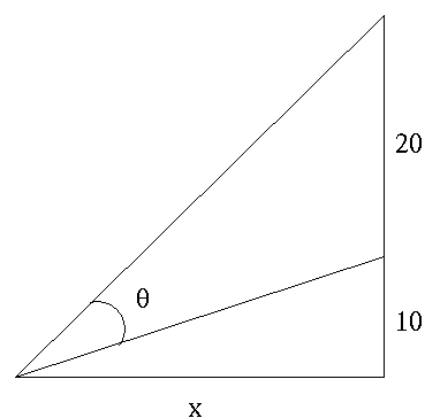
\includegraphics [scale=0.4] {movie_screen.png} \end{center}

\[ \tan s - t = \frac{\tan s - \tan t}{1 + \tan s \tan t} \]

Plugging in the values provided:
\[ \tan \theta = \tan s - t \]
\[ = \frac{30/x - 10/x}{1 + 300/x^2} \]
\[ = 20 \ \frac{x}{x^2 + 300} \]
We take the derivative and set it equal to zero.  We can ignore the leading factor of $20$, obtaining
\[ 0 = \frac{x^2 + 300 - 2x^2}{(x^2 + 300)^2} = \frac{-x^2 + 300}{(x^2 + 300)^2} \]

This is equal to zero when the numerator is zero, that is, when
\[ x = \pm \sqrt{300} \]
Since $x$ is a distance we take the positive square root.
\[ x = \sqrt{300} = 10 \sqrt{3} \]

The angles are worth working out.  The tangent of the lower angle $t$ is $1/\sqrt{3}$.  This is a right triangle with hypotenuse equal to $2$ and sine equal to $1/2$.  Therefore $t = \pi/6$.

The tangent of the entire angle $s$ is equal to $3/\sqrt{3} = \sqrt{3}$.  This is a right triangle with hypotenuse equal to $2$ and cosine equal to $1/2$.  Therefore $s = \pi/3$.  

Therefore the angle to the screen $\theta = s - t$ at the maximum is $\pi/6$ or 30 degrees.

\subsection*{folded paper}

Consider a piece of paper with the dimensions $6 \times 12$.  We pick up the lower right-hand corner and place it against the left side, folding to form a crease.

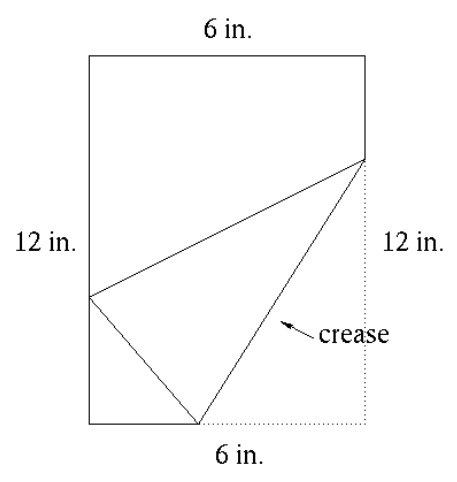
\includegraphics [scale=0.4] {folded_paper1.png}
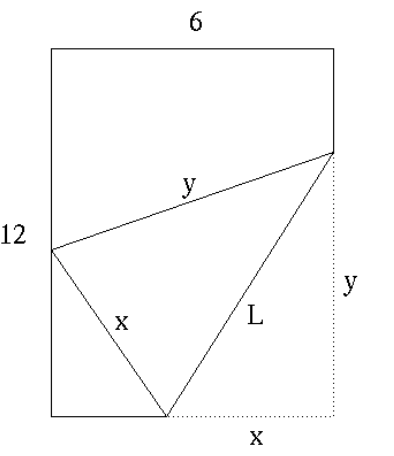
\includegraphics [scale=0.4] {folded_paper2.png}

The possible positions on the left-hand side to place that corner range from the bottom up to a distance 6 inches above the bottom.  The length of the crease is a variable, and and we wish to find the crease with the minimum length.

The variable distances can be labeled as shown on the right.  The length $L^2 = x^2 + y^2$.

I notice that the drawing is not properly scaled (the long dimension is too short).  In fact, the angle that the folded part makes on the left-hand side is a right angle.  After all, it is a corner of the original sheet, but also we have two congruent triangles, they must both be right triangles.

\begin{center} 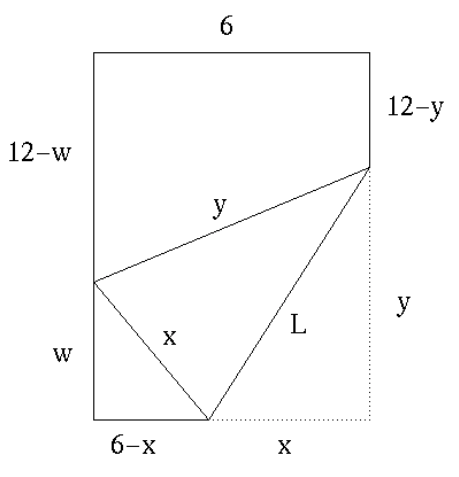
\includegraphics [scale=0.4] {folded_paper3.png} \end{center}
At this point, I notice that the problem can be re-scaled so the length of the paper is $2$ and the width is $1$, in order to simplify the arithmetic.  I have not re-done the drawings to reflect that yet, but our math will take advantage of it.

The range of the distance $x$ is $[1/2,1]$, while that for $y = [1,2]$.

We need to find a relationship between $x$ and $y$.  Start by labeling another variable distance $w$, as shown above.  

The connection that we need can be found by relating $x$, $y$ and $w$ to the total area of the paper.  We have two right triangles with sides $x$ and $y$ and total area $xy$.  

The other triangle has
\[ w^2 = x^2 - (1 - x)^2 \]
\[ = 2x - 1 \]
\[ w = \sqrt{2x - 1} \]
and area (we leave $w$ as it is for now).
\[ \frac{1}{2} (1-x) w  \]
We will need it later, so let's get the derivative of $w$ with respect to $x$
\[ \frac{dw}{dx} = \frac{1}{\sqrt{2x - 1}} = \frac{1}{w} \]

Last, we have a rhombus.  The average of the two vertical sides is 
\[ \frac{1}{2} (2 - w + 2 - y) = 2 - \frac{1}{2} (w + y) \]
and since the horizontal side is $1$, this is also equal to the area.

\subsection*{area calculation}

From the dimensions of the paper, the total area is $2$ and this is equal to the three triangles and the rhombus added together
\[ 2 = xy + \frac{1}{2} (1-x) w  + 2 - \frac{1}{2} (w + y)  \]
\[ 4 = 2xy + (1-x)w  + 4 - w - y \]
Cancel the $4$ and gather terms with $y$.  The left-hand side is
\[ y - 2xy =  -y(2x - 1) = -yw^2 \]
So
\[ -yw^2 = (1-x)w - w \]
Factor out one $w$
\[ -yw = (1 - x) - 1 = -x \]
\[ y = \frac{x}{w} \]

That's a nice simplification.  We can check that this is correct at one extreme.  When $x = w = 1$ the ratio is $1 = y$ and we see that is correct for the fold at 45 degrees.  At the other extreme we have $w = 0$ and the ratio is undefined.

And only now do I see that this calculation was unnecessary.  Draw the horizontal

\begin{center} 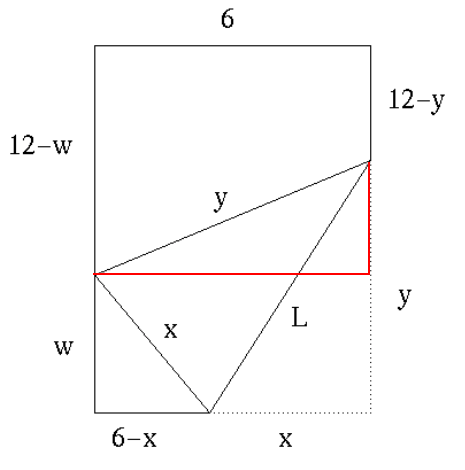
\includegraphics [scale=0.4] {folded_paper4.png} \end{center}

Can you see the similar triangles?  The angle between $w$ and $x$ is rotated by 90 degrees counter-clockwise to form the angle between the horizontal of length $1$ and $y$, so $w/x = 1/y$, which is exactly what we said.

Now, minimize $L$
\[ L = x^2 + y^2 \]
\[ = x^2 + \frac{x^2}{w^2} \]
Take the derivative:
\[ \frac{dL}{dx} = 2x + \frac{2xw^2 - 2wx^2 \cdot 1/w}{w^4} \]

\[ \frac{dL}{dx} = 2x + \frac{2x (2x - 1) - 2x^2}{(2x -1)^2} \]
Factor out $2x$ and set equal to zero:
\[0 = 1 + \frac{(2x - 1) - x}{(2x -1)^2} \]
\[ 0 = (2x - 1)^2 + x - 1 \]
\[ 4x^2 - 3x = 0 \]
Factor out another $x$
\[ 4x - 3 = 0 \]
\[ x = \frac{3}{4} \]
The minimum crease length occurs when $x$ is halfway along its range.

I found the last problem here:

\url{https://www.math.ucdavis.edu/~kouba/CalcOneDIRECTORY/maxmindirectory/MaxMin.html}


\end{document}  